
\chapter{Method of characteristics}
\label{app:char}

In this appendix, we present a general method to solve \textit{hyperbolic partial differential equations}, a class of equations to which conservation laws belong.
We believe it is best to see the method in action with an example. As we are interested in solving segregation equations, in this appendix we will solve a simplified version of the fully 3D segregation equation:
\begin{equation}
	u(z) \p{}{x} \phi - q \p{}{z} \phi(1-\phi) = 0
\end{equation}
This is the 2D version of our equation, in the stationary regime, and for the most simple velocity profile:
\begin{equation}
	\mathbf{v} = 
	\begin{pmatrix}
	u \\
	0 \\
\end{pmatrix}
\end{equation}
In this case, since we assume incompressibility, $u$ is a function of $z$ only.

\section{Characteristic curves}
The steady-state solution is a function of 2 variables: $ \phi = \phi(x, z)$. So the solution can be seen as the surface $ \phi - \phi(x,z) = 0$ of the 3D space $(x, z, \phi)$. 
\textit{Characteristics} are curves defined by $\phi = \Phi(x(s),z(s))$ lying on the solution surface, and satisfying
\begin{equation}
	\frac{d \Phi}{d s} = 0
\end{equation}
Using chain rule we have 
\begin{equation}
	\tot{x}{s} \p{\Phi}{x} + 
	\tot{z}{s}\p{\Phi}{z} = 0
\end{equation} 
and since $\Phi$ is lying on the solution surface,
\begin{flalign}
\tot{x}{s} = u \\
\tot{z}{s} =  - q(1- 2 \Phi)
\end{flalign}

So solving the segregation equation (and in fact, any conservation law) is equivalent to solving a system of ordinary differential equations, which is easier to do. Indeed we have at our disposal a number of tools to attack ordinary differential equations, whereas very few will work with partial differential equations such as conservation laws.


Rather than using a parameter $s$, we can directly express $z$ as a function of $x$, and since 
\begin{equation}
	\tot{z}{s} = \tot{x}{s} \frac{d z}{d x} 
\end{equation} 
we have
\begin{equation} \label{eq:charac}
	u \frac{d z}{d x} =  - q (1- 2 \Phi)
\end{equation}

This equation is known as the characteristic equation, because solving it will give us the equation of any characteristic curve lying on the solution surface. 
This is then sufficient to reconstruct the whole solution.

\section{Change of coordinates}

Of course, to solve the characteristic equation in our case, we need to know the explicit expression of the velocity $u$. But there is a clever way to get around this difficulty.
We note that since the flow is \textit{incompressible}, we can define the stream function $\psi$ as
\begin{align}
	\p{\psi}{x} = - w \\
	\p{\psi}{z} = u
\end{align}
In our case of course $w$ is zero, but this method is more general.

Now we remap the $z$ axis of the physical space using $\psi$. We we make the change of coordinate $z \leftarrow \psi$.
For example, let us choose a simple linear velocity profile:
\begin{equation}
	u(z) = \frac{U}{H} \left( z - \frac{H}{2} \right)
\end{equation}
with $z$ varying from 0 to $H$. The stream function is then
\begin{equation}
	\psi(z) = \frac{U}{2H} \left( z - \frac{H}{2} \right) ^2
\end{equation}
Note that $\psi$ takes the same value for 2 different values of $z$: $\psi(z) = \psi(H - z)$.
In other words, $z \rightarrow \psi(z)$ is not a bijection (and therefore not a good change of coordinates) on the interval $[0, H]$. But this is not a problem, it just means that we need to cut our interval by the middle, and solve separately for each half.

Back to the general solving of the characteristic equation, if we make the change of coordinates, we have using chain rule again,
\begin{equation}
	u\tot{z}{x} = \p{\psi}{z} \tot{z}{x} = \tot{\psi}{z}
\end{equation}
so, in the new system of coordinates, we can solve for the characteristic curves without knowing explicitly the velocity field!
Indeed now we have
\begin{equation}
		\tot{\psi}{z} =  - q (1- 2 \Phi)
\end{equation}
and since $\Phi$ is constant along the characteristic curve,
\begin{equation}
	\psi(x) = - q x (1-2\Phi) + \psi_0
\end{equation}
And that is it! We just solved our problem.
Of course it is just a trick: the velocity profile explicit dependence is hidden in $\psi$, as we need to know it to actually do the change of coordinate. But this trick is exceedingly useful to understand the global structure of the solution without having to prescribe a velocity field, as we will see now.

\section{Shock waves and jump condition}
We said that we can decompose our surface solution as a set of curves, called characteristic curves. This is the essence of the method of characteristics. 
What happens if two such curves cross? In that case the method can no longer be used, and in fact the solution is no longer a function, but becomes a discontinuous \textit{distribution}.

In the physical space $(x, z)$  two regions where the solution $\psi$ is a function are separated by a discontinuity in $\psi$, a \textit{jump} in the concentration.
The equation of the interface can be calculated using the so-called Rankine-Huginiot jump condition. We will not give here a demonstration of this formula as the derivation in itself is not specially enlightening, but I can be found for example in \cite{leveque}.

In our case, the condition is
\begin{equation}
	\tot{\psi}{x} = q \left( \phi^+ + \phi^- - 1\right)
\end{equation}
where $\phi^+$ and $\phi^-$ are the concentrations at each side of the interface.

This jump condition and the characteristic equation is all we need to know to understand the full structure of the solution. But of course, we need to prescribe a boundary condition to start with.

\section{Structure of the solution}

We will solve our equation on a bounded domain. We won't give any details on the chosen velocity profile. We will just prescribe the value of the $\phi$ at the left boundary of our domain. Let us suppose it is a constant (ie we start with an homogeneous mixture of small and large particles) and call it $\phi_0$. The particles will be advected to the right by the velocity field, and the concentration will evolve as $x$ increases. 

How? Well, we know from experiments and from our intuition that after some time (ie from $x$ sufficiently large) the mixture will be fully segregated, ie a jump will separate a region of large particles ($\phi=0$) and a region of small particles ($\phi=1$). Similarly, the initial region of concentration $\phi_0$ will be separated from the upper region of large particles by a jump. If we use the jump condition, with $\phi^- = \phi_0$ and $\phi^+ = 0$, we have
\begin{equation}
	\psi^u(x) =  \psi^u_0 - q x (1-\phi_0)
\end{equation}
similarly, for the jump separating the lower region of small particles ($\phi^+=1$) and the homogeneous region ($\phi^- = \phi_0$),
\begin{equation}
	\psi^l(x) =q x \phi_0
\end{equation}

These two shocks will begin immediately to form, at $x=0$. They will join at some point called the triple point, because it is at the interface between 3 regions: the homogeneous region, the large particles region and the small particles region. The whole structure is summed up in the figure \ref{1}.

\begin{figure}[htp]
\centering
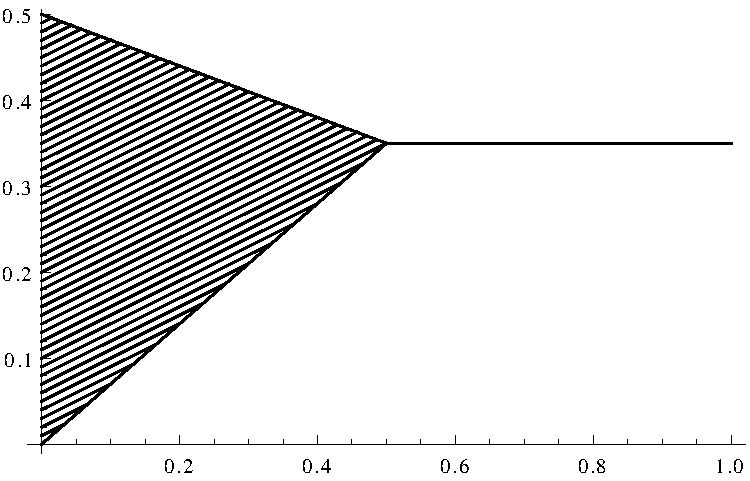
\includegraphics[scale=1.00]{/home/nicolas/git/reports/M1/vector/characteristics.pdf}
\caption{Structure of the solution of the simplified segregation equation, with an homogeneous concentration input. The characteristics are shown, as well as the jumps (in bold).}
\label{1}
\end{figure}